\section{Experimental Evaluation}
\label{sec:evaluation}

This section presents the experimental evaluation of the implemented chess
engine. The evaluation pursues the central question of this thesis: where lies
the sweet spot between invested search time and decision quality, and how do the
individual search refinements shift this trade-off? The strongest empirical
effect is produced by null-move pruning, which is therefore examined in detail,
while the Principal Variation Search parameter sweep yields a deliberate null
result that is reported and explained rather than hidden. All measurements are
based on a common position suite and a uniform scoring methodology, so that the
individual experiments remain directly comparable.

\subsection{Research Objectives}
\label{subsec:research_objectives}

The experimental evaluation addresses the following research questions:

\begin{itemize}
    \item \textbf{Playing strength:} how strong is the engine under realistic
    tournament time controls when compared to a fixed reference opponent?
    \item \textbf{Null-move pruning:} how does null-move pruning affect reachable
    depth, node throughput, transposition table behavior, and move quality across
    time budgets?
    \item \textbf{Transposition table size:} from which table size onward does
    the available memory stop limiting the search?
    \item \textbf{Time-to-quality and depth-versus-time:} how do reachable depth
    and move quality develop as the time budget increases, and where does
    additional time stop paying off?
    \item \textbf{PVS parameter sweep:} which combination of minimum scouting
    depth (\texttt{PvsMinDepth}) and number of fully searched moves
    (\texttt{PvsScoutAfterMove}) yields the best ratio of cost reduction to move
    quality?
    \item \textbf{Search tree reuse:} how much depth does a persistent
    transposition table gain over the course of a game compared to starting each
    search from an empty table?
    \item \textbf{Move stability:} at which search depth does the best move
    stabilize, so that deeper search no longer changes the decision?
\end{itemize}

The playing-strength question establishes an absolute reference point, while the
remaining questions characterize time-dependent decision making directly and
quantify the effect of the individual search refinements.

\subsection{Experimental Setup}
\label{subsec:common_setup}

Unless stated otherwise, all experiments share the following configuration.

\paragraph{Hardware and Build.}
All measurements were conducted on a MacBook Pro with an Apple M3 Pro processor
and 18\,GB of RAM. The engine was compiled in release mode and executed as a
single-threaded process. Apart from the parameter that is varied in a given
experiment, all engine options were kept at their defaults throughout.

\paragraph{Position Suite.}
The experiments use a fixed suite of 309 positions
(\texttt{tests/data/stockfish-bench-all.epd}), derived from the position set that
Stockfish uses for its own benchmark. Each configuration is measured with three
repetitions per position to average out scheduling noise, and reported figures
are means over positions and repetitions.

\paragraph{Time Budgets.}
Time-dependent experiments sweep a fixed set of per-move budgets of
$10, 25, 50, 100, 250, 500, 1000, 2000$, and $5000$\,ms. This range spans from
very short thinking times, where only shallow searches are possible, to budgets
that reach depths well into the middlegame.

\paragraph{Quality Scoring.}
Because the positions have no known ground-truth best move, move quality is
measured against a strong reference. For every position, Stockfish is run to a
fixed depth of 20 to obtain both a reference best move and a reference
evaluation. Two metrics are derived from this reference:
\begin{itemize}
    \item \textbf{Centipawn loss (CPL):} the difference, in centipawns and from
    the perspective of the side to move, between the reference evaluation of
    Stockfish's preferred move and the reference evaluation of the move actually
    played by the engine. Lower is better; a value of $0$ means the engine played
    a move of equal reference value.
    \item \textbf{Agreement:} the fraction of positions in which the engine's
    chosen move coincides exactly with Stockfish's reference move.
\end{itemize}
CPL is the primary quality metric, as it also credits moves that differ from the
reference move but are of comparable value; agreement is reported as a
complementary, stricter indicator.

\paragraph{Benchmark Harness.}
All experiments are driven by the dedicated benchmarking harness in the
\texttt{bench/} directory, which records for each search, among others, the
completed depth, selective depth, node and quiescence-node counts, the number of
PVS re-searches and null-move cutoffs, transposition table statistics, and the
elapsed time. The raw per-search records are written to CSV files and aggregated
offline, which keeps measurement and analysis reproducible. Each file also stores
the commit hash of the engine it was produced with, so every table in this
chapter can be traced back to a specific state of the implementation.

\paragraph{Correctness of the Move Generator.}
All results rest on the assumption that the engine generates and applies moves
correctly. This is verified with \emph{perft}~\cite{cpw_perft}, the standard
correctness test for
chess engines: for a set of reference positions, the number of leaf nodes of the
full game tree is counted up to a fixed depth and compared against published
values. Any error in move generation, in make--unmake, or in the handling of
castling, en-passant and promotion changes these counts and is thus detected. The
engine reproduces the reference values for all tested positions and depths.

\subsection{Playing Strength (Engine versus Engine)}
\label{subsec:engine_eval}

To place the engine on an absolute strength scale, it is evaluated in
head-to-head matches against a fixed reference opponent under tournament
conditions. The matches are played through the CuteChess framework, with a
development build of Stockfish as the reference opponent. To obtain a comparison
in the target strength range, Stockfish is restricted through its built-in
strength limitation (\texttt{UCI\_LimitStrength} with a nominal target of
2000\,Elo), a single search thread, and a 32\,MB hash; Helix likewise runs
single-threaded with a 32\,MB hash and otherwise default settings. Both engines
play a classical time control of five minutes per side with a 0.5\,second
increment.

To obtain a fair and diverse sample, the games are opened from a balanced opening
book (\texttt{8moves\_v3}), with each opening played once from either side so
that both engines receive identical starting positions as White and Black. In
total 400 games are played with alternating colors. Clearly decided games are
adjudicated to keep the match tractable: a game is scored as won once both
engines agree on an evaluation beyond $\pm 600$ centipawns for several
consecutive moves, and as drawn once the evaluation stays within $\pm 10$
centipawns for several moves in the late middlegame. All games run on the Apple
M3 Pro machine described in \cref{subsec:common_setup}. Playing strength is
reported as an Elo difference derived from the match result, together with the
likelihood of superiority (LOS) and the draw ratio.

\cref{tab:elo_results} summarizes the match.

\begin{table}[ht]
\centering
\begin{tabular}{@{}lr@{}}
\toprule
Metric & Value \\ \midrule
Games played & 400 \\
Score (W--L--D) & 288--76--36 \\
Elo difference & $+205.0 \pm 37.8$ \\
Likelihood of superiority & $100.0\,\%$ \\
Draw ratio & $9.0\,\%$ \\ \bottomrule
\end{tabular}
\caption{Match result of Helix against Stockfish limited to a nominal 2000\,Elo,
over 400 games at a 5+0.5 time control.}
\label{tab:elo_results}
\end{table}

Helix wins the match decisively, with an Elo difference of roughly $+205$ points
and a likelihood of superiority of $100\,\%$. The advantage holds with both
colors: Helix scores $138$--$40$--$22$ as White ($74.5\,\%$) and
$150$--$36$--$14$ as Black ($78.5\,\%$), so it remains clearly stronger even
without the first-move advantage. The moderate draw ratio of $9.0\,\%$ indicates
that most games are decided rather than drawn.

It should be emphasized that this is a \emph{relative} result. The reference
engine was deliberately weakened, and Stockfish's \texttt{UCI\_LimitStrength}
provides only a nominal Elo target that does not map directly onto established
rating lists; it also weakens play partly by introducing random inaccuracies
rather than uniformly. The reported difference therefore characterizes Helix's
strength relative to this specific, equally configured opponent, not an absolute
rating.

\subsection{Effect of Null-Move Pruning}
\label{subsec:eval_nmp}

Null-move pruning (\cref{subsec:null_move_pruning}) is the search refinement with
the largest measured effect on the engine. It was evaluated by running the full
time-budget sweep twice, once with pruning enabled and once disabled, on the
common suite. \cref{tab:nmp_depth_cpl} reports the reachable depth and the
centipawn loss for both configurations.

\begin{table}[ht]
\centering
\begin{tabular}{@{}rcccc@{}}
\toprule
 & \multicolumn{2}{c}{Completed depth (ply)} & \multicolumn{2}{c}{Centipawn loss} \\
\cmidrule(lr){2-3}\cmidrule(lr){4-5}
Budget (ms) & without NMP & with NMP & without NMP & with NMP \\ \midrule
10   & 3.67 & 3.91 & 60.2 & 61.9 \\
25   & 4.29 & 4.65 & 58.9 & 60.7 \\
50   & 4.86 & 5.30 & 57.1 & 56.0 \\
100  & 5.37 & 5.96 & 57.2 & 60.2 \\
250  & 6.04 & 6.81 & 54.6 & 55.7 \\
500  & 6.52 & 7.53 & 56.8 & 55.0 \\
1000 & 7.08 & 8.16 & 55.5 & 52.4 \\
2000 & 7.55 & 8.79 & 49.2 & 50.3 \\
5000 & 8.09 & 9.43 & 43.8 & 44.4 \\ \bottomrule
\end{tabular}
\caption{Reachable depth and centipawn loss with and without null-move pruning,
averaged over 309 positions and three repetitions per budget.}
\label{tab:nmp_depth_cpl}
\end{table}

The clearest and most robust effect is on search depth: null-move pruning reaches
a greater depth at \emph{every} one of the nine budgets, and the gap widens with
more time, from $+0.24$\,ply at 10\,ms to a full ply ($8.16$ versus $7.08$) at one
second and $+1.34$\,ply at five seconds. This confirms that skipping provably
weak subtrees lets the engine invest the saved effort into depth.

This additional depth is not bought at the cost of node throughput. At the
one-second budget the engine reaches about $1.69$ million nodes per second with
pruning versus $1.61$ million without, so pruning is if anything slightly faster
per node as well. What does change is the transposition table hit rate, which
drops from $0.208$ to $0.158$ at one second: by pruning subtrees, the search
visits a larger number of \emph{distinct} positions and re-visits known entries
less often. The hit rate is therefore best read as a symptom of the search shape
rather than as a quality target in itself.

The effect on move quality, however, does not follow the depth gain, and this is
reported here without smoothing. Across the nine budgets the pruning
configuration achieves a lower centipawn loss in only three cases (50\,ms,
500\,ms and 1000\,ms) and a higher one in the remaining six; averaged over all
budgets the difference amounts to $+0.37$\,cp in favour of the configuration
\emph{without} pruning, which is well inside the noise of three repetitions. The
largest single gain for pruning occurs at one second ($52.4$ versus $55.5$\,cp),
the largest loss at 100\,ms ($60.2$ versus $57.2$\,cp).

Taken together, this is the central and somewhat sobering observation of this
experiment: null-move pruning reliably buys depth, but the additional depth does
not translate into measurably better moves. A full extra ply at one second leaves
move quality statistically unchanged. This is the first direct piece of evidence
for the thesis question, and it is examined further in
\cref{subsec:eval_ttq,subsec:eval_move_stability}: beyond a certain point the
engine is not limited by how deep it searches, but by what its evaluation can
distinguish. \cref{fig:quality_vs_depth,fig:search_nps} visualize the quality and
the node throughput across budgets.

\begin{figure}[ht]
\centering
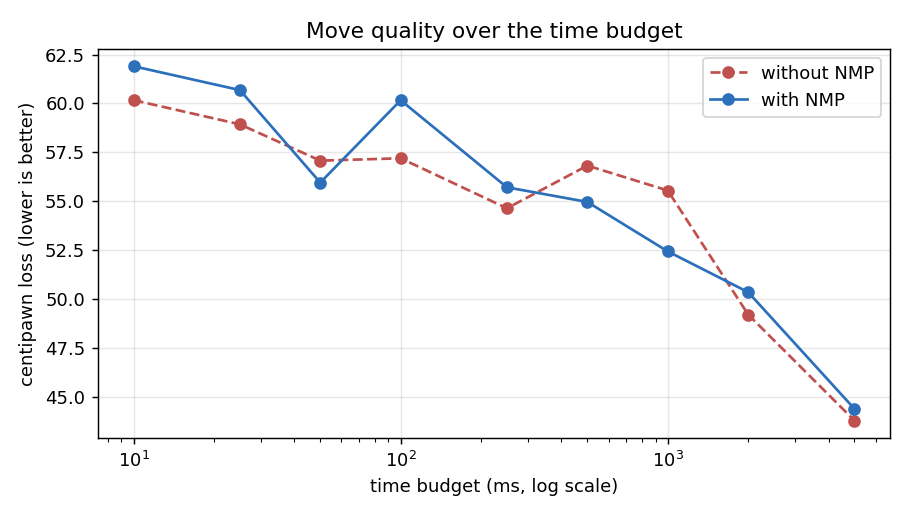
\includegraphics[width=0.8\linewidth]{figures/quality_vs_depth.png}
\caption{Centipawn loss as a function of the reached depth (and thus time budget)
with and without null-move pruning.}
\label{fig:quality_vs_depth}
\end{figure}

\begin{figure}[ht]
\centering
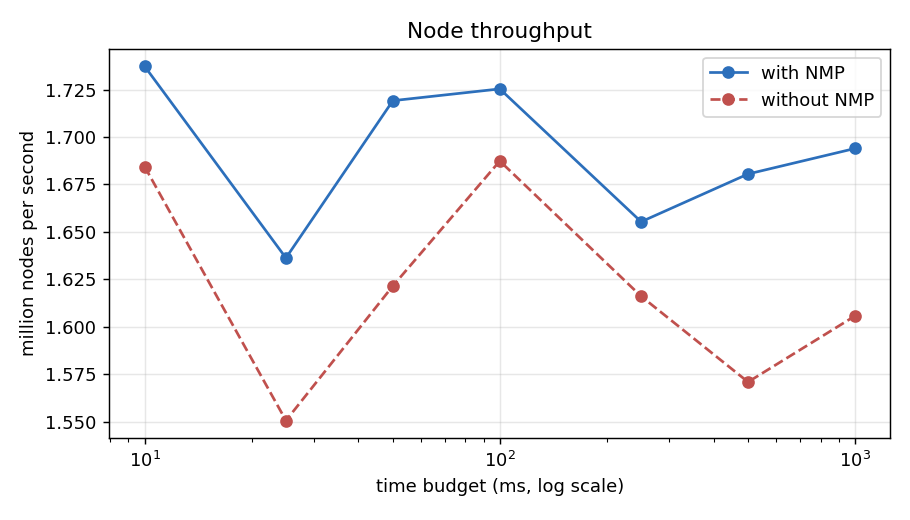
\includegraphics[width=0.8\linewidth]{figures/search_nps.png}
\caption{Node throughput (nodes per second) across time budgets with and without
null-move pruning.}
\label{fig:search_nps}
\end{figure}

\subsection{Transposition Table Size}
\label{subsec:eval_tt_size}

The transposition table trades memory for search efficiency: a larger table
retains more previously computed positions but consumes more memory. To determine
a sensible default, the table size was swept over $1, 4, 16, 64$, and $256$\,MB
at a fixed one-second budget, with null-move pruning enabled.
\cref{tab:tt_size} reports the reachable depth, the eviction rate (the share of
stores that overwrite an entry of a different position), and the hit rate.

\begin{table}[ht]
\centering
\begin{tabular}{@{}rccc@{}}
\toprule
Table size (MB) & Completed depth (ply) & Eviction rate & Hit rate \\ \midrule
1   & 7.75 & 0.610 & 0.104 \\
4   & 8.01 & 0.263 & 0.134 \\
16  & 8.14 & 0.076 & 0.153 \\
64  & 8.18 & 0.019 & 0.161 \\
256 & 8.18 & 0.005 & 0.163 \\ \bottomrule
\end{tabular}
\caption{Effect of transposition table size at a one-second budget, averaged over
309 positions and three repetitions.}
\label{tab:tt_size}
\end{table}

Only the smallest table has a measurable negative effect: at 1\,MB the search
loses roughly half a ply of depth ($7.75$ versus $\approx 8.2$) while more than
$60\,\%$ of all stores evict a foreign entry, so useful information is displaced
before it can be reused. From 16\,MB onward the curve flattens; the difference
between 64\,MB and 256\,MB is within noise, even though the eviction rate keeps
falling. For the target time controls the search therefore stops being
memory-bound well below 32\,MB, which justifies the default hash size used
elsewhere in this work.

\subsection{Time-to-Quality and Depth-versus-Time}
\label{subsec:eval_ttq}

The per-budget measurements in \cref{tab:nmp_depth_cpl} also answer the
time-to-quality and depth-versus-time questions directly. Reachable depth grows
smoothly and predictably with the budget, roughly one additional ply per
doubling of time in the tested range, which reflects the exponential relationship
between depth and node count discussed in \cref{sec:preliminaries}.

Move quality, in contrast, improves far less smoothly. Over the whole range from
10\,ms to 5000\,ms, a factor of 500 in thinking time, the centipawn loss of the
pruning configuration falls only from about $62$ to $44$\,cp, and it does so
non-monotonically: the curve rises again at 100\,ms and at 2000\,ms before
continuing downwards. Put differently, the first $250$\,ms buy roughly three
plies of depth but barely six centipawns of quality, while the last step from
2000 to 5000\,ms buys a further $0.6$\,ply and six more centipawns.

This is the central observation behind the thesis question. Depth and decision
quality are not proportional: additional search time reliably converts into
depth, but only weakly into better moves. The engine typically finds a move of
comparable quality early and spends the remaining time confirming it, which is
consistent with the move stability results in
\cref{subsec:eval_move_stability}. The practical sweet spot therefore lies where
the depth curve is still rising steeply while the quality curve has already
flattened, which for this engine and suite is reached around one second per move.

\subsection{Distribution of Move Quality}
\label{subsec:eval_outliers}

All centipawn losses reported so far are means over the suite, and that summary
turns out to hide the actual behavior of the engine. The distribution of the
per-position loss is strongly skewed: at a one-second budget the \emph{median}
loss is $2$\,cp while the \emph{mean} is $52.4$\,cp. In $49.0\,\%$ of all
positions the engine plays exactly the move Stockfish prefers, and in $66.3\,\%$
it stays within $25$\,cp of it. At the other end, $6.9\,\%$ of the positions
(21 of 306) exceed $200$\,cp, and the fifteen worst positions alone account for
$46.3\,\%$ of the entire mean. The average is therefore not a description of the
typical case, it is a description of a small number of failures.

This also changes how the time-to-quality result of \cref{subsec:eval_ttq} should
be read. Measured by the median, additional time helps clearly and monotonically:
the median loss falls from $16$\,cp at 10\,ms over $7$\,cp at 100\,ms to $2$\,cp
at one second. The mean, dominated by the outliers, barely moves over the same
range. The engine does not gradually get better at every position, it solves more
and more positions outright while a hard residue stays unsolved regardless of the
budget.

The outliers share a recognizable profile. Positions with a loss above $200$\,cp
hold on average $13.8$ pieces, against $19.5$ for the well-played ones, and a
third of them are endgames with ten pieces or fewer. Three positions reach the
scoring cap of $1000$\,cp, meaning Stockfish sees a forced mate the engine misses
entirely. A typical example is the pawn endgame
\texttt{8/1p3pp1/7p/5P1P/2k3P1/8/2K2P2/8 w}, in which the engine plays
\texttt{g4g5} instead of the winning \texttt{f5f6}.

This is a direct consequence of the evaluation function discussed in
\cref{subsec:eval_limitations}. Material and piece-square tables describe a
middlegame reasonably well, but they encode nothing about passed pawns,
opposition or king activity, the very concepts that decide sparse endgames. In
such positions no attainable search depth compensates for what the evaluation
cannot express, which is consistent with these positions being exactly the ones
that never stabilize in \cref{subsec:eval_move_stability}. It also explains why
the depth gained through null-move pruning does not show up in the mean: the
positions where extra depth would matter are the ones limited by evaluation
knowledge, not by depth.

\subsection{PVS Parameter Sweep}
\label{subsec:eval_pvs_sweep}

Principal Variation Search exposes two tunable parameters, the minimum scouting
depth (\texttt{PvsMinDepth}) and the number of leading moves searched with the
full window (\texttt{PvsScoutAfterMove}). To determine whether these parameters
offer a worthwhile tuning gain, a full grid of $6 \times 5 = 30$ configurations
(\texttt{PvsMinDepth} $1$ to $6$, \texttt{PvsScoutAfterMove} $1$ to $5$) was
evaluated on the full suite at a one-second budget with null-move pruning
enabled. \cref{tab:pvs_sweep} lists a representative selection.

\begin{table}[ht]
\centering
\begin{tabular}{@{}ccccc@{}}
\toprule
\texttt{PvsMinDepth} & \texttt{PvsScoutAfterMove} & Depth (ply) & Nodes & Re-searches \\ \midrule
1 & 1 & 8.16 & 1\,534\,720 & 104.1 \\
2 & 1 & 8.15 & 1\,531\,145 & 52.2 \\
3 & 1 & 8.16 & 1\,539\,544 & 29.2 \\
6 & 5 & 8.09 & 1\,531\,458 & 3.2 \\ \bottomrule
\end{tabular}
\caption{Representative configurations from the PVS parameter sweep (one-second
budget). The default configuration is \texttt{PvsMinDepth}\,$=2$,
\texttt{PvsScoutAfterMove}\,$=1$.}
\label{tab:pvs_sweep}
\end{table}

The sweep is a deliberate null result: across all 30 configurations the completed
depth stays between $8.09$ and $8.16$\,ply and the node count between $1.52$ and
$1.55$ million, a spread of about $1.8\,\%$ that is within measurement noise. No
configuration offers a meaningful improvement over any other.

The reason is visible in the re-search column. The whole point of the scouting
parameters is to control the trade-off between the savings of the cheap
null-window scout and the cost of the occasional full-window re-search when the
scout fails high. In this engine that trade-off barely materializes: even the
most aggressive configuration triggers only about $104$ re-searches over roughly
$1.5$ million nodes, and the most conservative one only about $3$. The existing
move ordering (transposition-table move, MVV-LVA captures, killer moves, and the
history heuristic) is already good enough that the first move is almost always
the best, so the null-window scout almost always holds and there is little
re-search cost left for the parameters to tune away. As a side observation, the
transposition table hit rate correlates weakly with the number of re-searches
($0.158$ at $104$ re-searches versus $0.144$ at $3$), which again confirms that
the hit rate reflects the shape of the search rather than being an independent
quality target. Consequently, the default configuration
(\texttt{PvsMinDepth}\,$=2$, \texttt{PvsScoutAfterMove}\,$=1$) is retained, as no
setting in the sweep improves upon it.

\subsection{Search Tree Reuse}
\label{subsec:eval_tree_reuse}

The second refinement of this thesis is the reuse of previously explored search
trees through a persistent transposition table (\cref{subsec:tree_reuse}). Its
value cannot be measured on isolated positions, since it only materializes when
consecutive searches are related, so this experiment replays complete games
instead. The 30 games are taken from the match of \cref{subsec:engine_eval}, and
every position of every game is searched with a fixed budget of 500\,ms, once in
each of two modes: in \emph{keep} the table survives the whole game, which is the
engine's normal behavior, and in \emph{clear} it is wiped before every single
search. Both runs see identical positions under identical budgets, so the
difference between them is precisely the value of resuming the old tree.
\cref{tab:tree_reuse} reports the aggregate over all 2256 plies.

\begin{table}[ht]
\centering
\begin{tabular}{@{}lccc@{}}
\toprule
Mode & Completed depth (ply) & TT hit rate & Nodes \\ \midrule
TT cleared each move & 7.23 & 0.136 & 758\,979 \\
TT kept (tree reuse) & 7.52 & 0.152 & 772\,368 \\ \bottomrule
\end{tabular}
\caption{Effect of search tree reuse over 30 complete games (2256 plies) at a
500\,ms budget per move.}
\label{tab:tree_reuse}
\end{table}

Keeping the table yields $+0.28$\,ply on average at an unchanged time budget,
together with a hit rate that rises from $0.136$ to $0.152$, i.e., by about
$12\,\%$ relative. A paired comparison per position shows how this average comes
about: in $69\,\%$ of all plies both modes reach exactly the same depth, in
$28\,\%$ the persistent table reaches deeper, and only in the remaining few does
the cleared table win. Tree reuse thus does not speed up every single search, it
provides a head start in those positions where the new root actually lies inside
the previously explored tree.

That reading is supported by the development over the course of a game, shown in
\cref{fig:tree_reuse}. The gain grows from $+0.16$\,ply in the opening
(plies 0--15) over $+0.22$ in the middlegame to $+0.39$ in the endgame
(ply 41 onwards), where the hit rate also climbs to $0.207$ versus $0.178$. With
fewer pieces on the board, positions transpose more often and a larger share of
the stored tree remains reachable, so the retained information keeps paying off
increasingly as the game progresses.

\begin{figure}[ht]
\centering
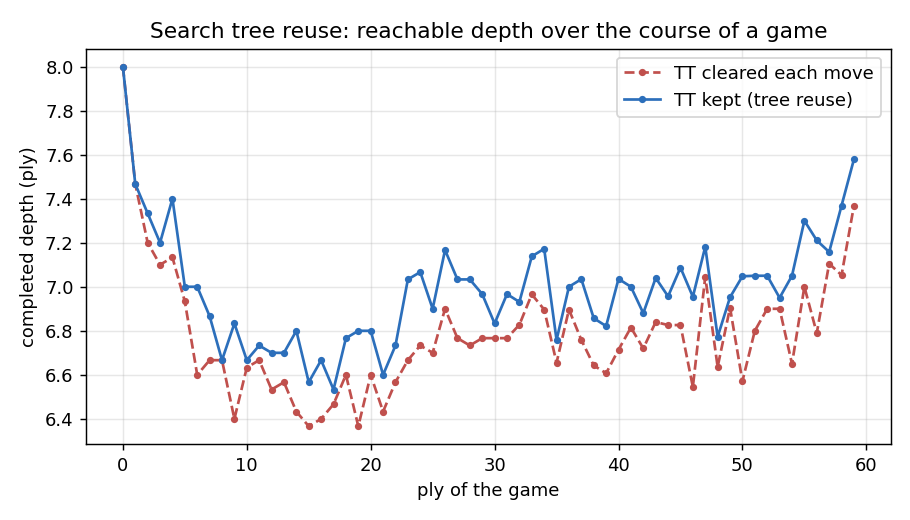
\includegraphics[width=0.8\linewidth]{figures/tree_reuse.png}
\caption{Reachable depth per ply of the game, averaged over 30 games, with the
transposition table kept versus cleared before every search.}
\label{fig:tree_reuse}
\end{figure}

Compared to null-move pruning, the effect is smaller in absolute terms ($+0.28$
versus a full ply), but it comes at no cost whatsoever: no search parameter is
changed, nothing is pruned away, and no accuracy is traded. The engine merely
stops discarding what it has already computed.

\subsection{Move Stability}
\label{subsec:eval_move_stability}

The final question concerns move stability: at which depth does the engine's
chosen move settle, so that deeper search no longer changes the root decision?
This is measured with a single iterative-deepening search per position. Because
iterative deepening already produces a best move at every completed depth, one
search yields the full sequence of root moves without repeated re-searching. Each
position is searched under a fixed budget of 20 million nodes with the
transposition table cleared beforehand, so that the depth sequence reflects one
self-contained search. A node budget is used instead of a fixed target depth
because it bounds the cost per position and, being independent of wall-clock time,
is unaffected by other load on the machine.

For each position the \emph{stabilization depth} is defined as the smallest depth
from which the root move matches the move of the deepest completed iteration and
does not change again \emph{within the searched range}. Positions whose move still
changes at the deepest searched depth are counted as not yet settled within the
budget. Of the 309 positions, 306 produced a usable move sequence, reaching a mean
depth of $10.1$ plies. \cref{fig:move_stability} shows the cumulative distribution
and \cref{tab:move_stability} lists selected thresholds.

This definition can only observe what happens inside the budget, which has to be
kept in mind when reading the numbers. A move that survives until the last
completed iteration might still change one ply deeper, and the evidence for a late
stabilization is necessarily thinner than for an early one: a position that
settles at depth 3 and is searched to depth 11 confirms that move eight more
times, whereas one that settles at depth 10 out of 11 confirms it once. The
measurement quantifies this directly. On average a stabilized move is confirmed by
$4.3$ further iterations (median 3), but for $22.2\,\%$ of the positions the move
changed in the very last iteration, which is why those are reported as unsettled
rather than as stabilized at the final depth. Restricting the analysis to the 178
positions whose move is confirmed by at least three further iterations shifts the
median stabilization depth down to 3 plies, with $87\,\%$ settled by depth 6.
That subset is itself selective, since it excludes late stabilizers by
construction, so the two views bracket the effect rather than replacing one
another: the reported figures are an upper bound on the depth actually needed.

\begin{figure}[ht]
\centering
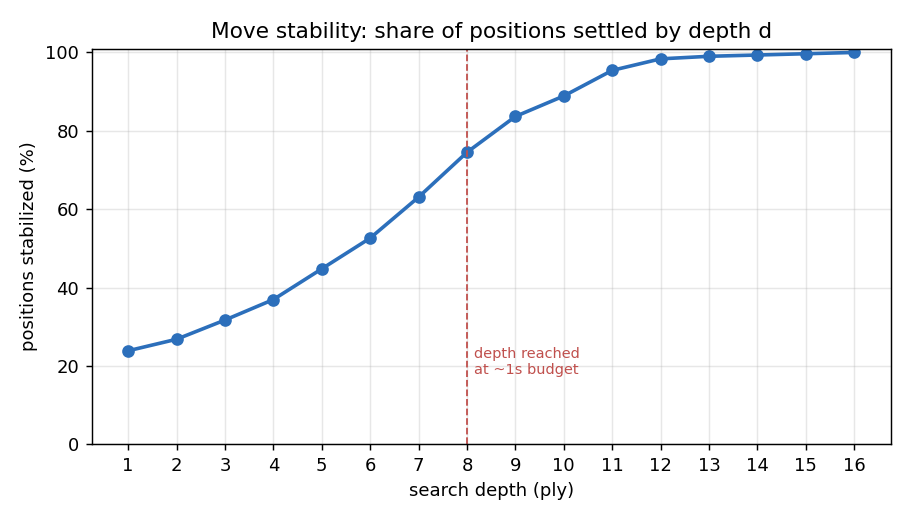
\includegraphics[width=0.8\linewidth]{figures/move_stability.png}
\caption{Share of positions whose root move is settled by depth $d$. The dashed
vertical line marks the depth ($\approx 8$) the engine reaches at a one-second
budget.}
\label{fig:move_stability}
\end{figure}

\begin{table}[ht]
\centering
\begin{tabular}{@{}rr@{}}
\toprule
Depth $d$ (ply) & Positions settled by $d$ \\ \midrule
2  & $26.8\,\%$ \\
4  & $36.9\,\%$ \\
6  & $52.6\,\%$ \\
8  & $74.5\,\%$ \\
10 & $88.9\,\%$ \\ \bottomrule
\end{tabular}
\caption{Cumulative share of positions whose best move has stabilized by a given
depth (306 positions, 20-million-node budget).}
\label{tab:move_stability}
\end{table}

The root move settles early for most positions: the median stabilization depth is
6 plies, and $23.9\,\%$ of positions never change their move at all. By depth 8,
roughly the depth the engine reaches at a one-second budget
(\cref{tab:nmp_depth_cpl}), three quarters of all positions have already locked in
their final move. This is the central evidence for the sweet-spot argument of this
thesis: beyond this point additional search keeps increasing depth but only rarely
changes the decision.

At the same time, the effect is not uniform. Roughly one position in five
($22.2\,\%$) still changes its move at the deepest depth searched, i.e., remains
unsettled even around depth 10 and beyond. These are the tactically sharp
positions in which deeper search still changes the decision, and they are the
only ones for which the extra ply bought by null-move pruning
(\cref{subsec:eval_nmp}) can pay off at all. Since they make up only a fifth of
the suite, an across-the-board gain in depth is diluted accordingly, which
explains why the substantial depth gain of null-move pruning leaves the average
centipawn loss unchanged. Move stability is therefore concentrated: the majority of decisions are
made cheaply and early, while a hard minority keeps rewarding deeper search.

\subsubsection{Stability in Evaluation Rather Than in the Move}
\label{subsubsec:eval_eps_stability}

Judging stability by the identity of the move has a blind spot: a switch between
two moves of equal value counts as instability, while converging on a
consistently poor move counts as success. To separate these cases, every move of
every iteration was additionally scored against the reference engine, and a
position is called \emph{$\varepsilon$-stable} from the smallest depth at which
its centipawn loss stays below $\varepsilon$ for all deeper iterations.
\cref{tab:eps_stability} contrasts the two criteria and \cref{fig:eps_stability}
shows the corresponding curves.

\begin{table}[ht]
\centering
\begin{tabular}{@{}lcccc@{}}
\toprule
Criterion & Positions reaching it & Median depth & By depth 6 & By depth 8 \\ \midrule
Move identity            & $100\,\%$  & 6 & $52.5\,\%$ & $74.4\,\%$ \\
$\varepsilon = 0$\,cp    & $52.5\,\%$ & 4 & $35.1\,\%$ & $43.9\,\%$ \\
$\varepsilon = 20$\,cp   & $66.9\,\%$ & 2 & $49.5\,\%$ & $60.0\,\%$ \\
$\varepsilon = 50$\,cp   & $78.4\,\%$ & 1 & $63.6\,\%$ & $72.1\,\%$ \\ \bottomrule
\end{tabular}
\caption{Move stability judged by move identity versus by evaluation, for 305
scored positions. Percentages refer to the whole set, so positions that never
reach the criterion are included in the denominator.}
\label{tab:eps_stability}
\end{table}

\begin{figure}[ht]
\centering
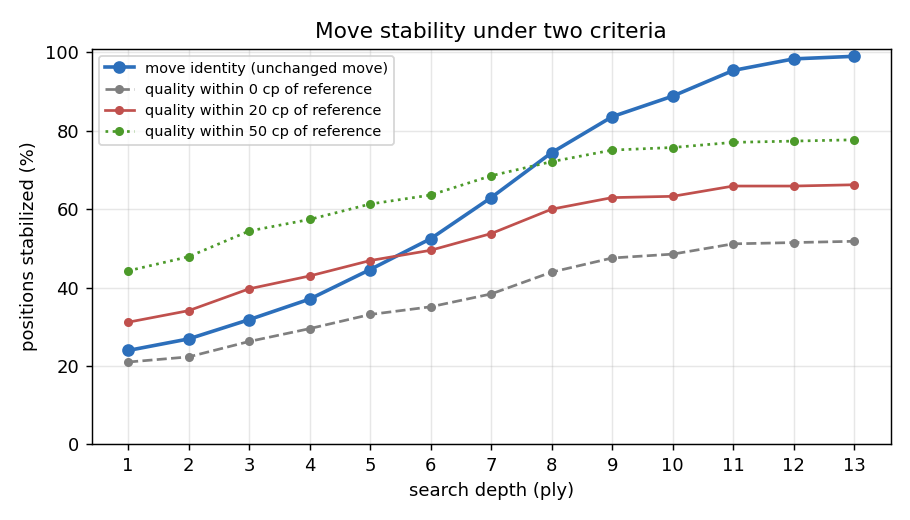
\includegraphics[width=0.8\linewidth]{figures/move_stability_eps.png}
\caption{Cumulative share of positions considered stable by depth $d$, judged by
the identity of the move and by its distance to the reference evaluation.}
\label{fig:eps_stability}
\end{figure}

The two criteria disagree in both directions, and the curves cross at around
depth 6. Below that, judging by evaluation reports \emph{more} stability: at
depth 3 already $39.7\,\%$ of the positions are within 20\,cp, against $31.8\,\%$
whose move has settled. The engine reaches a decision of adequate quality earlier
than it settles on one particular move, since part of the apparent instability is
merely alternation between moves of comparable value.

Above depth 6 the relation reverses, and this is the more consequential half. By
move identity, $88.9\,\%$ of the positions have settled by depth 10; measured
against the reference evaluation, only $63.3\,\%$ are within 20\,cp, and
$33.1\,\%$ never reach that margin at any depth. These are not positions in which
the move keeps changing: their move does settle, but it settles on something
poor, with a mean loss of $120$\,cp at the deepest iteration. Fourteen of the 21
worst positions from \cref{subsec:eval_outliers} are among them.

Both readings therefore support the same conclusion from opposite sides. Where
the engine is able to find a good move, it finds it early, earlier than the
move-identity criterion suggests. Where it is not, the search converges
confidently on the wrong answer. Stability of the move is thus a necessary but
not a sufficient indicator of a settled decision.

It is worth asking whether these positions would simply need more depth. The data
argue against it. Both groups are searched to the same average depth of $10.1$
plies under the shared node budget, so the difference is not one of search effort.
What differs is how much that effort achieves: comparing the first half of each
search to the second, and excluding the final iteration that defines the grouping,
the loss falls by $36.5$\,cp on average for the positions that do converge, but
only by $5.4$\,cp for those that do not. The same picture emerges when comparing
shallow to intermediate depths, where the converging positions gain $41.5$\,cp and
the others $21.9$\,cp. Additional depth is therefore not without effect on the
difficult positions, but it is roughly half to one seventh as effective, and it
starts from a worse level. Extrapolating the observed rate, the remaining gap of
over $100$\,cp would not be closed by the few plies that are realistically
attainable. The bottleneck lies in the evaluation, which cannot express what
distinguishes these positions, and a search that optimizes a misleading objective
more thoroughly does not arrive at a better move.
